\documentclass[12pt]{article}
 
\usepackage[margin=1in]{geometry} 
\usepackage{amsmath,amsthm,amssymb}
\usepackage{graphicx}
\usepackage{hyperref}
\usepackage{fancyhdr}
\usepackage{enumitem}
\usepackage{textcomp}

\pagestyle{fancy}

%\lhead{\href{https://github.com/hanuka24/ActMonitoringLocalizationApp}{Link} to our repository}

\begin{document}
 
\title{Mobile Computing, Lab}
\author{Hannah Brunner, Markus Gallacher}

\maketitle


\section{Introduction}

The aim of the course was to implement a smartphone app on Android, which utilizes and processes on-phone sensor data. Two assignments had to be delivered:

The first task was an activity monitoring application using the KNN algorithm. Accelerometer data is sensed for a given time window and features such as mean or min/max value are extracted. These values can then be compared to prior recorded and labeled samples to derive the current activity. Further details are explained in Section \ref{sec:activitymonitoring}.

Second, an indoor localization application using a particle filter had to be implemented. Therefor, a map of the ITI buildings' second floor was given. For localization, a number of particles is spread on the map in random manner and moved according the users' walking direction. The filtering of unlikely paths respectively particles should reveal the users' current position. The algorithm is described in Section \ref{sec:localization}.

The source code of the app is available on GitHub \cite{repo}. 

\section{Implementation}
\subsection{Main App}
We combined both tasks (activity monitoring and localization) into a single app. It consists of four activities:
\begin{enumerate}
	\item \textbf{MainActivity:} Shows the home screen, which appears at start of the app (see Figure \ref{fig:main}) and contains buttons to start the desired activity.
	\item \textbf{TrainActivity:} Records and stores accelerometer data associated with desired activity, which is used during activity monitoring (see Section \ref{sec:train}).
	\item \textbf{MonitorActivity:} Monitors and displays the user's current activity (see Section \ref{sec:monitoring}).
	\item \textbf{LocalizationActivity:} Implementation of indoor localization using particle filter (see Section \ref{sec:localization}).
\end{enumerate}

\begin{figure}
	\centering
	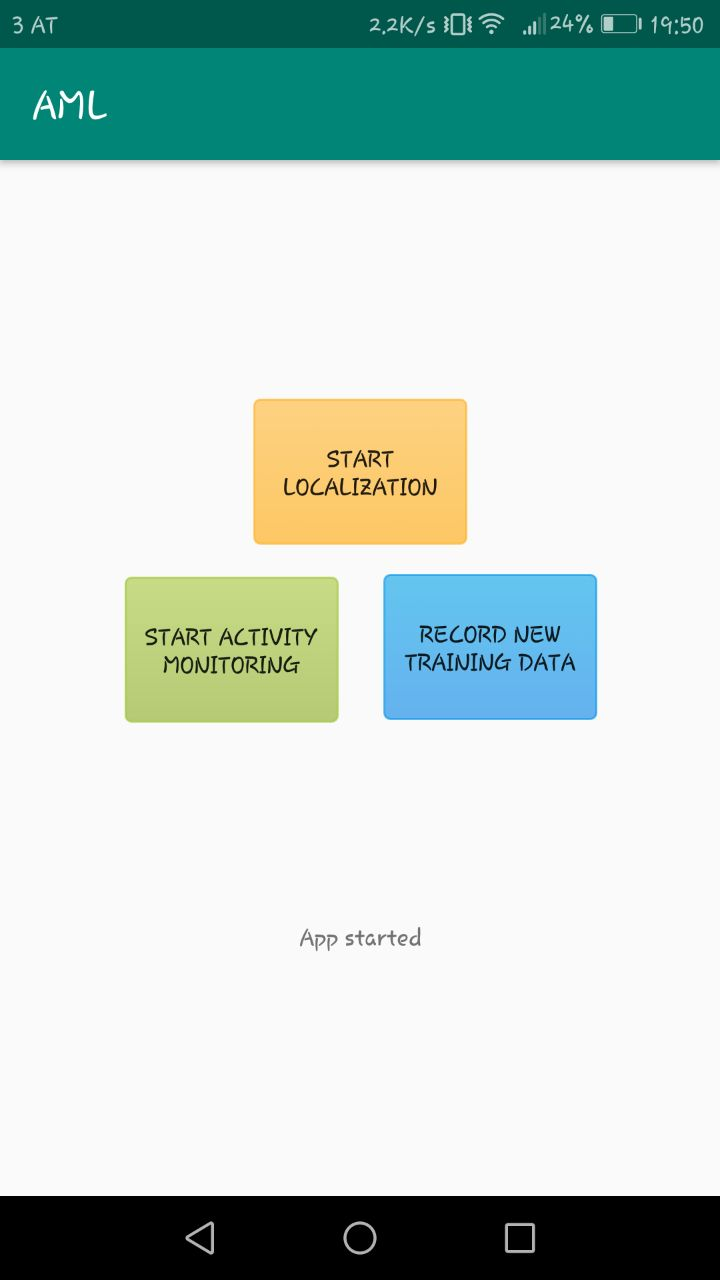
\includegraphics[width=140px]{images/main.jpeg}
	\caption{Home screen}
	\label{fig:main}
\end{figure}

\subsection{Activity Monitoring}\label{sec:activitymonitoring}
The Activity Monitoring is split into two activities, one collects training data and stores it into a file locally. The other activity monitors the sensors and uses the kNN algorithm to classify the user's motion.

\subsubsection{Background: Activity monitoring using KNN}

\subsubsection{Train Activity} \label{sec:train}
This activity enables the user to collect training data for the monitoring activity. 1 of 4 activities are currently implemented, however any activity can be trained, only the label would mismatch at the moment.
\\
The user needs to press one of the activities and perform the motion. The accelerometer data is sampled over a predefined window and the timestamp, mean of the x, y and z axis as well as the minimum and maximum of the euclidean distance is stores in a local .txt file. The most dominant frequency is also stored but it is currently not used as it lowers the recognition accuracy.
\\
If a faulty measurement was recorded the user can delete the last entry or delete the whole .txt file.

\begin{center}
  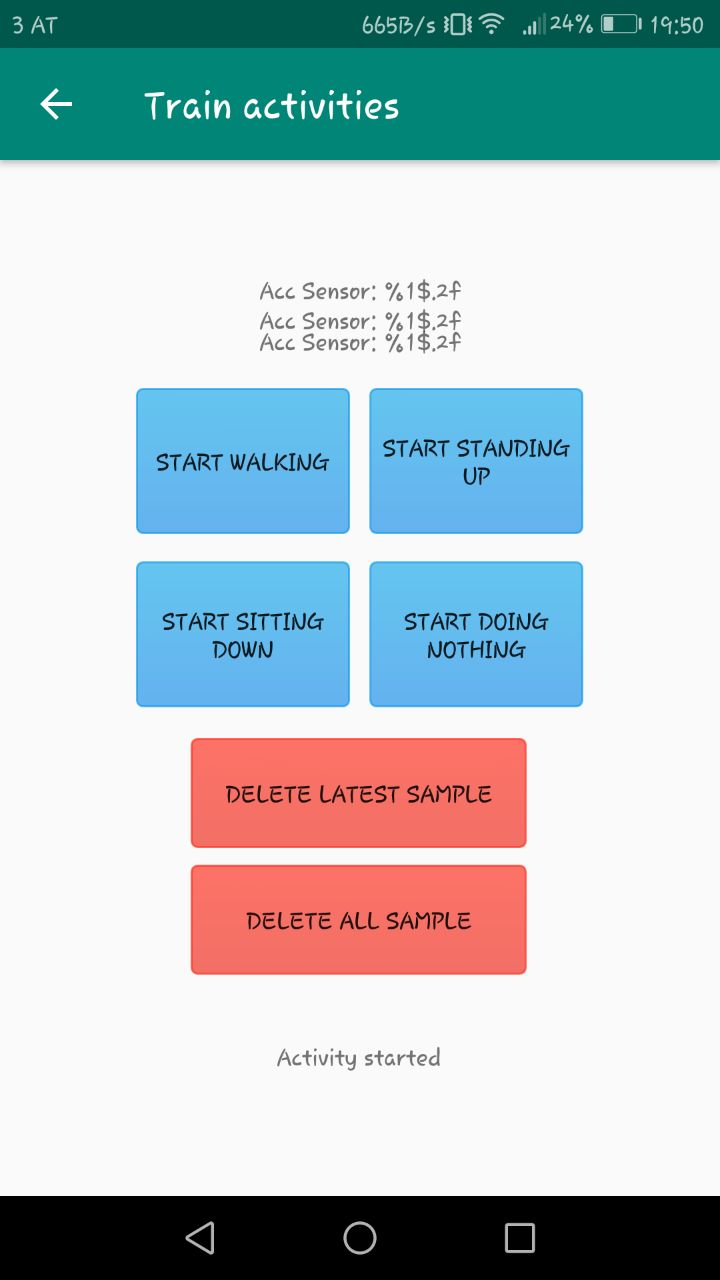
\includegraphics[width=140px]{images/train_activity}
\end{center}

\pagebreak
 
\subsubsection{Monitoring} \label{sec:monitoring}


The second activity tries to classify the activity currently performed by the user. When the button is pressed, the accelerometer data is sampled with the same window size as the training data. 
\\
Then a kNN algorithm finds the nearest neighbours by calculating the euclidean distance of the averaged coordinates to each training record and selecting the k closest ones. 
\\
Then we classify the neighbours by weighting each label and adding the weights if a label occurs more than once. This gives us a probability of how certain we are of our match. The recognized activity is displayed together with the probabilities for each of our 4 predefined activities.
\\
When the "continuous monitoring" box is ticked, this prediction process (sample, kNN, classify) is repeated endlessly.

\begin{center}
  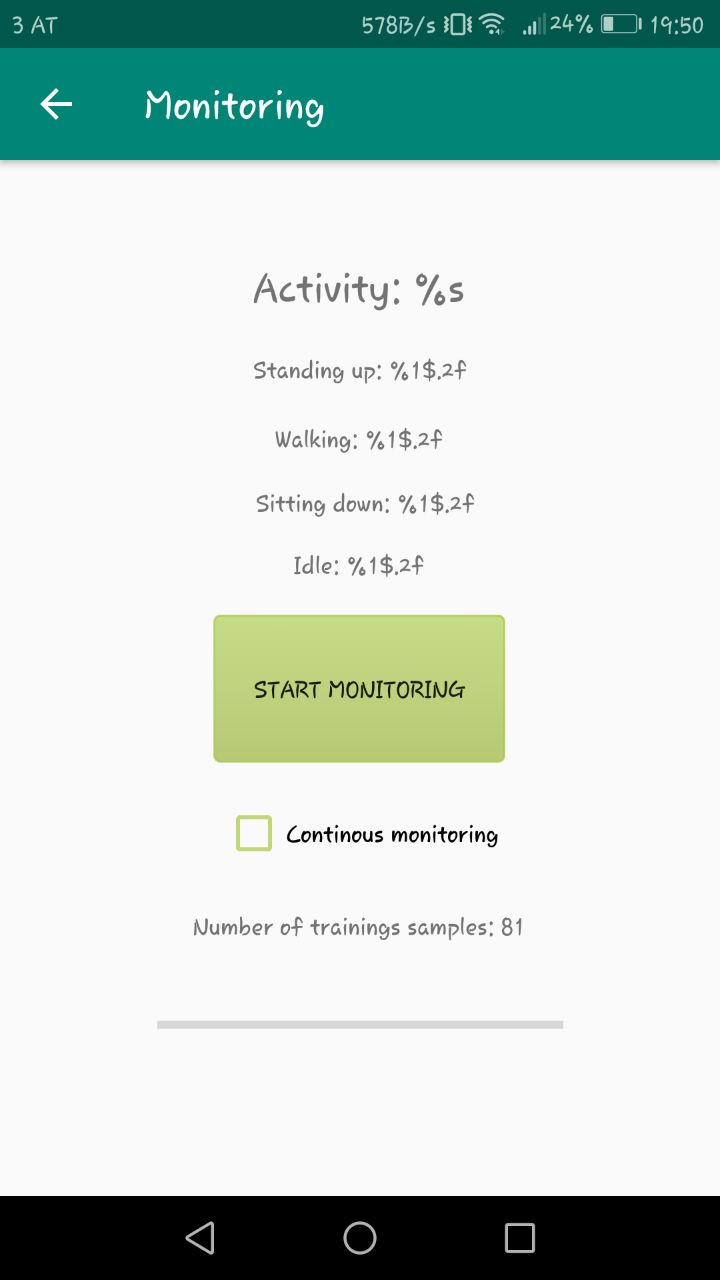
\includegraphics[width=140px]{images/monitoring.jpeg}
\end{center}

\pagebreak

\subsubsection{Limitation/Challenges}

%Python script, accuracy etc.

\subsection{Localization} \label{sec:localization}

\subsubsection{Background: Particle Filter} \label{sec:particlefilter}
Particle filters are a rather easy and very suitable approach for indoor localization. The basic idea is to spread a high number of particles randomly in the environment. If the user moves, the particles move in the same direction. Particles, which violate physical constraints (e.g. walk into a wall) are a deleted and thus, only a set of possible particles will survive to give the user's location. \\
Localization using a particle filter is an iterative process consisting of the following steps:
\begin{enumerate}
	\item \textbf{Spread N particles:} An arbitrary, but high number (5000-1000) of particles are spread on the map.
	\item \textbf{Move:} If the user moves, the same movement is applied on all particles. To compensate for sensing errors, a variance in movements length and direction is added.
	\item \textbf{Sense:} It is checked, if physical constraints are violated (particles walking through a wall). If so, the particles' weight (likelihood) is set to zero.
	\item \textbf{Resample:} To avoid particle depletion, particles are regenerated each cycle. Thus, the number of particles stays constant. Resampling is done by replacement. Particles with weight equal to zero will disappear, while particles with weight greater than zero might have multiple copies.
	\item \textbf{Compute position:} The position can be obtained by finding the point with the highest particle density.
\end{enumerate}
The repitition of steps 2 to 5 will eventually lead to convergence and reveal the current position.


\subsubsection{Implementation}
\subsubsection*{GUI}
As shown in Figure \ref{fig:localization}, the localization activity displays a map of the ITI building's first floor, text fields to report the users movement, an arrow indicating the user's current orientation and three buttons to 
\begin{itemize}[noitemsep,topsep=0pt]
	\item move a single particle
	\item init particles and start localization
	\item show the walls of the building on the map (mainly debug purposes)
\end{itemize}

\begin{figure}
	\centering
	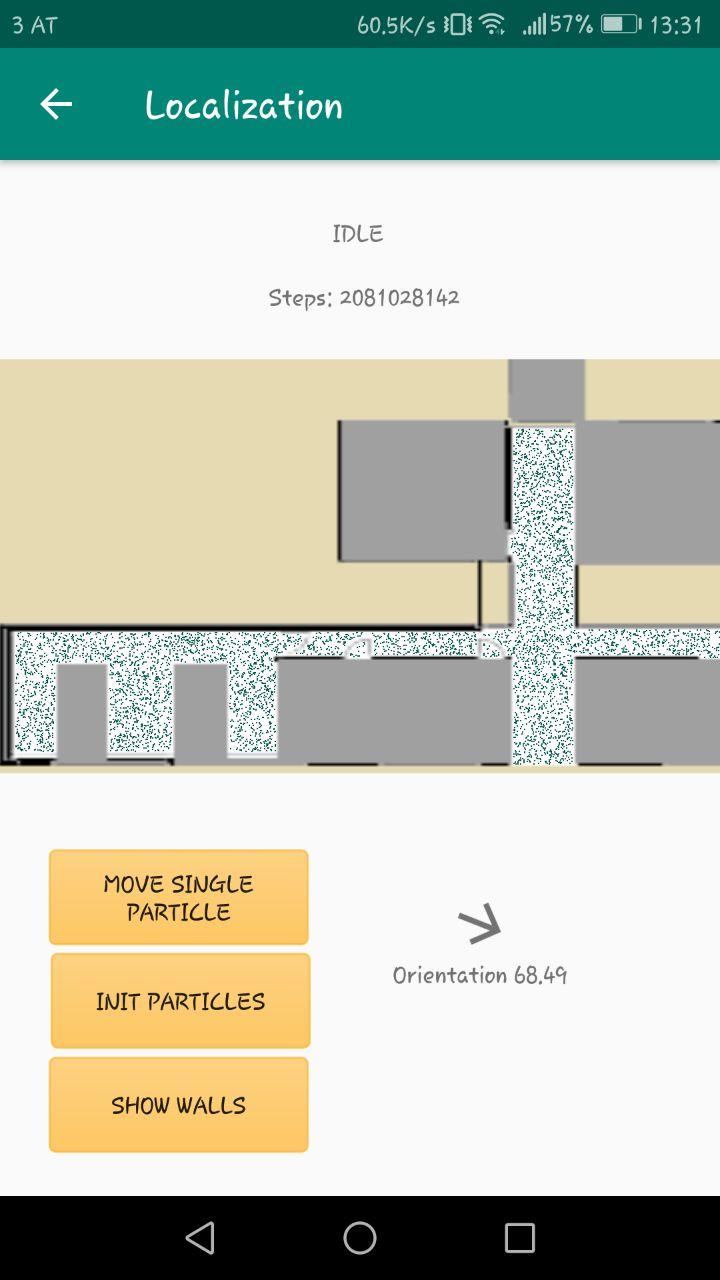
\includegraphics[width=140px]{images/localization.jpeg}
	\caption{UI of localization activity. 1) Main screen after initializing. 2) After a few steps. 3) After convergence. }
	\label{fig:localization}
\end{figure}

\subsubsection*{Movement detection}\label{sec:movement}
In order to detect the user's movement to create an appropriate movement model, we utilized the smartphone's build in accelerometer and magnetic sensor. The movement detection is implemented in a background service, similar to the implementation of \ref{sec:monitoring}.\\
The user's orientation is retrieved using the Android method \textit{getOrientation}, which utilizes the acceloremeter and magentic sensor. Since the value is quite inaccurate, the median value of the measurement while walking is used.\\
To detect if the user started respectively stopped walking, the %TODOO: explain and cite reference (olga's page)\\

The travelled distance was approximated by measuring the walking time and assuming a constant walking speed of the user.


\subsubsection*{Particle Filter}
In the following, we will give some details about the implementation of steps 1-5, explained in \ref{sec:particlefilter}
\begin{enumerate}
	\item \textbf{Spread N particles:} We chose N = 6000, which gave a reasonable tradeoff between computation time and accuracy. 
	\item \textbf{Move:} The movement is sensed as explained in \ref{sec:movement} and we add a variance of \textpm 20cm for step width and \textpm 20\textdegree~ for the orientation angle.
	\item \textbf{Sense:} To check if particles moved out of the valid area, we introduced walls in a hardcoded manner. We then compute the line between the last position and the newly computed position. If the lines of the wall and movement intersect, a violation of the physical constraints is detected.\\
	The initial idea with wall pixels turned out to be too slow for real-time computing.
	\item \textbf{Resample:} For resampling, an easy approach was implemented. Each deleted particle is replaced by a randomly chosen valid one.
	\item \textbf{Compute position:} To compute the final position, we calculate the median of x and y coordinates indepentendly. 
\end{enumerate}

\subsubsection{Limitations/Challenges}
The main challenge was the inaccuracy of the orienatation measurements. During the debugging process, we discovered big problems when passing by metal doors or walls. Outdoors, it was much more accurate.



\bibliographystyle{IEEEtran}
\bibliography{refs}
The rest of theoratical content is based on the lecture notes (\url{https://github.com/osaukh/mobile_computing_lab/}). Other ressources related to the implementation can be found in the source code.



\end{document}